% Citeed equations
% references
% verificar se se responde a tudo



\documentclass[letterpaper, 10 pt, conference]{ieeeconf}

\usepackage[utf8]{inputenc}
\usepackage{amssymb}
\usepackage{amsmath}
\usepackage{array}
\usepackage{breqn}
\usepackage{xcolor}
\usepackage{float}
\usepackage{hyperref}

\usepackage{biblatex}
\addbibresource{references.bib}

\setlength{\abovedisplayskip}{7pt}
\setlength{\belowdisplayskip}{6pt}
\usepackage{graphicx}
\usepackage{caption}
\usepackage{subcaption}
\usepackage{siunitx}
\usepackage{longtable}
\usepackage{comment}
\usepackage[margin=1.5cm]{geometry}
\newcommand{\MATLAB}{\textsc{Matlab\textsuperscript{\tiny\textregistered}\hspace{1ex}}}
\newcommand{\simulink}{\textsc{Simulink\textsuperscript{\tiny\textregistered}\hspace{1ex}}}

\title{\LARGE \bf Linear State Feedback Control -- Inverted Pendulum}

\author{\textbf{Group 15}: Leonardo Pedroso (89691), Miguel Graça (90142), Tomás Bessa (90200), Inês Ferreira (90395)\\
Professor Pedro Batista and Professor João Miranda Lemos
}

\begin{document}

\maketitle
\pagestyle{empty}

\begin{abstract}
The aim of this project is to design a control solution for an inverted pendulum, which is a nonlinear system. It is modeled by a linear time invariant (LTI) system about the equilibrium point corresponding to the upright position. The approach followed consists of the design of a state feedback controller and a state observer to maintain the pendulum in the upright position and track piece-wise constant signals with the angle of the horizontal bar. The proposed control solution is validated via extensive simulations including nonlinear effects and other sources of nonideal dynamics.
\end{abstract}

\section{Introduction}
The project report is organized as follows. In Section \ref{sec:car} the plant is characterized and analyzed in terms of of its: i) dynamic modes, their origin, and effects on the control solution design; ii) observability; iii) controllability; and iv) frequency response. In Section \ref{sec:ctr}, the regulation problem is addressed assuming full-state feedback is available. In Section \ref{sec:obs}, a state observer is designed to provide state estimates to the previously designed controller, which are then cascaded making use of the Separation Theorem. In Section \ref{sec:sim}, nonlinear effects are studied and their effects are taken into account in the design of both the controller and the observer. In Section \ref{sec:trck}, the control solution is extended to the tracking problem. Finally, Section \ref{sec:concl} presents the main conclusions of this project.

\section{Plant Characterization}\label{sec:car}
The plant consists of an inverted pendulum. The pendulum is attached at the base to a horizontal bar that can be rotated in the horizontal plane by a DC motor. There are also two sensors that measure the angles of both bars with respect to a reference direction. The plant is depicted in Fig. 1. 
\begin{figure}[h]
    \centering
    \includegraphics[scale=0.1]{figures/ROTPEN-graphics.png}
    \caption{QUANSER rotary inverted pendulum \cite{balula2016nonlinear}.}
\end{figure}

The control strategy synthesis approach followed in this project is for systems described by linear models. Although the plant being studied is nonlinear, its dynamics can be linearized about an equilibrium point, which in this case is the upright position of the pendulum, which describes the behavior of the plant well for small deviations in relation to the equilibrium. The linearized model is, thus, given by
\begin{equation*}
\begin{cases}
    \dot{\mathbf{x}} = \mathbf{Ax}+\mathbf{B}u\\
    \mathbf{y} = \mathbf{Cx}
    \end{cases}\:,
\end{equation*}
where $\mathbf{x}:= [\alpha\;\dot{\alpha}\;\beta\;\dot{\beta}\;i]^T$, $\alpha$ is the angle of the horizontal bar, $\beta$ is the angle of the pendulum in relation to the upright position, $i$ is the current in the DC motor, $u\in \mathbb{R}$ is the motor input signal, and $\mathbf{A},\mathbf{B}$, and $\mathbf{C}$ are matrices or appropriate dimensions. 

Before proceeding with the controller implementation, it is important to characterize the system in terms of its: i) dynamic modes, their origin, and effects on the controller design; ii) observability; iii) controllability; and iv) frequency response. These aspects are addressed in this section, making use of the LTI system that is obtained linearizing the nonlinear dynamics of the plant about the upright position of the pendulum.

\subsection{Dynamic modes}\label{sec:dynModes}
First, the dynamic modes of the open-loop system are analyzed, from which conclusions can be made regarding its stability. It is well known that the poles of the system are given by the eigenvalues of matrix $\mathbf{A}$. These are presented in Table \ref{tb:ol_poles}. It is now of interest to analyze each mode and comment on its origin, and aspects to consider in the controller design.

\begin{table}[h]
    \centering
    \caption{Poles of open-loop system.}
    \begin{tabular}{cccc}
         \hline
         Pole & Damping & $\omega$ (rad/s) & Time constant (s) \\\hline
   0.00e+00 &   -1.00e+00 &      0.00e+00    &           $+\infty$  \\
 -7.37e+02   &  1.00e+00  &     7.37e+02      &    1.36e-03    \\
 -1.94e+01  &   1.00e+00   &    1.94e+01  &        5.16e-02    \\
 -5.76e+00  &   1.00e+00   &    5.76e+00      &    1.74e-01   \\ 
  7.00e+00   & -1.00e+00  &     7.00e+00      &   $-$ \\
        \hline
    \end{tabular}
    \label{tb:ol_poles}
\end{table}
\begin{comment}
\begin{table}[h]
    \centering
    \begin{tabular}{|c|c|}
         \hline
        Eigenvalue 1 & -737.3184  \\
         \hline 
        Eigenvalue 2 & -19.3673 \\ 
         \hline
        Eigenvalue 3 & -5.7612 \\
         \hline
        Eigenvalue 4 & 0 \\ 
         \hline
        Eigenvalue 5 & 6.9974 \\
        \hline
    \end{tabular}
    \caption{Eigenvalues of Matrix A}
    \label{A_eig}
\end{table}
\end{comment}

First, the fastest pole ($p = -737$ rad/s) is a real pole associated with the dynamics of the DC motor. Thus, the motor dynamics are modeled as a first order low pass system with a characteristic time of $1.36$ ms. Given that this mode is very stable and fast, when compared with the pendulum dynamics, it does not require much attention in the controller or observer design stages. Second, the second fastest pole ($p = -19.4$ rad/s) is associated with the relation between the current in the DC motor and the angular velocity of the horizontal bar. Its effect is noticeable, but it is still almost one order of magnitude faster than the pendulum dynamics. Third, there is a pole at the origin, which corresponds to integrator dynamics. It is associated with the angle $\alpha$ of the horizontal bar, whose dynamics are an integrator of the angular velocity of the bar. As it is discussed in Sections \ref{sec:sim} and \ref{sec:trck}, the existence of this pole on the open-loop dynamics of the plant allows for several beneficial properties such as rejection of some disturbances and robustness to model parameter identification uncertainty. Finally, the pair of poles ($p = -5.76$ rad/s and $p = 7.00$ rad/s) are associated with the inverted pendulum dynamics. It is possible to prove this association upon writing the differential equation that models an inverted pendulum with friction for small angles $\beta$ in relation to the equilibrium position
\begin{equation}\label{eq:sysPendulum}
    I\ddot{\beta} = mgl_{cm}\beta-\gamma_f\dot{\beta}\:,
\end{equation}
where $I$ is the moment of inertia about the pivot, $m$ is the mass, $l_{cm}$ is the distance from the pivot to the center of mass, and $\gamma_f$ is a coefficient of friction. The poles of the second order system described by \eqref{eq:sysPendulum}, obtained for reasonable values of the parameters and low coefficient of friction are two real poles, one stable and another unstable, whose absolute value is similar, which is consistent with the poles obtained. From an intuitive perspective, the existence of an unstable pole is expected as the inverted pendulum is naturally unstable in the upright position. One of the goals of the control strategy devised in this project is, thus, to stabilize the dynamics of the inverted pendulum.
\begin{comment} % Fui copianddo as frasese reformulando ... abaixo está o original [LEo]
The fastest pole (-737.3184) is expected to come from the motor dynamics (as DC motors are very fast in their actuation). The pole at -19.3673 is expected to be associated with some sort of function of torque and the motor's current, $i$.
stability is checked. Considering the nature of the inverted pendulum, the system should be unstable. A simple approach to verify this is to analyze the eigenvalues of matrix A. Because A is a 5x5 matrix, 5 eigenvalues are expected. The following table shows the obtained eigenvalues, using the Matlab function \textit{eig}.
Matrix A has three negative eigenvalues, a zero eigenvalue, and a
positive eigenvalue. The existence of the positive eigenvalue is expected as the analyzed system (inverted pendulum) is naturally unstable. These eigenvalues correspond to the poles of the system and it is important to understand the role of each eigenvalue on the system's dynamics.
The poles at -5.7612 and 6.9974 are expected to be associated with the pendulum dynamics and the angle $\beta$ (given that the pendulum is a second-order system and is unstable). Finally, the pole at the origin is an integrator, expected to be associated with $\alpha$. Throughout the report, it will be shown that these predictions are correct.
\end{comment}

\subsection{Controllability}\label{sec:ctrolbty}
It is well known that a continuous-time system is completely controllable iff the controllability matrix
\begin{equation*}
    \mathcal{C} := \begin{bmatrix} \mathbf{B} & \mathbf{AB}& \dots & \mathbf{A}^{n-1}\mathbf{B}
    \end{bmatrix}\:,
\end{equation*}
where $n$ is the order of the system, is full rank. After computing the controllability matrix and its rank, it is confirmed that it is full rank, thus the system is completely controllable. This result is, by no means, obvious, since there is only one input and the state has five components, two of which are two mechanical degrees of freedom of the physical system. It is well known that this result guarantees that there is a state feedback gain such that the closed-loop poles are wherever one desires. In Section \ref{sec:freq_resp}, with the analysis of the frequency response of the system, an intuitive explanation on controllability is also provided.
\begin{comment} % Original - fui copiando [Leo]
Next, to check the system's controllability, the Matlab function \textit{ctrb} is applied to the matrix pair (A,B). As A is a 5x5 matrix and B is a 1x5 vector, the controllability matrix is a 5x5 matrix. Its rank is 5, equal to the number of columns. This implies that the system is completely controllable, i.e., from any
initial state, it is possible to reach the origin in finite time.
\end{comment}

\subsection{Observability}\label{sec:obsvlty}
It is well known that a continuous-time system is completely observable iff the observability matrix
\begin{equation*}
    \mathcal{O} := \begin{bmatrix} \mathbf{C} \\ \vdots \\ \mathbf{C}\mathbf{A}^{n-1}
    \end{bmatrix}\:,
\end{equation*}
where $n$ is the order of the system, is full rank. This test is applied to two distinct cases: i) the output is only the pendulum angle $\beta$, \textit{i.e.} 
\begin{equation*}
    \mathbf{C} := \begin{bmatrix} 0 & 0 & 1 & 0 & 0\end{bmatrix}\:;
\end{equation*}
and ii) the output is both angles of the bars, $\alpha$ and $\beta$, \textit{i.e.},
\begin{equation}\label{eq:Cused}
    \mathbf{C} := \begin{bmatrix} 1 & 0 & 0 & 0 & 0\\ 0 & 0 & 1 & 0 & 0\end{bmatrix}\:.
\end{equation}
After computing the observability matrix for both these cases, in the first case, it is not full rank, but in the second case it is. Therefore, the system is not completely observable if the output is only the pendulum angle $\beta$. It is necessary to measure the angle of the horizontal bar $\alpha$ as well to infer the evolution of the state variables. In Section \ref{sec:freq_resp}, with the analysis of the frequency response of the system, the observability of the system is also discussed, and the reason for the lack of complete observability in the first case is explained.

\begin{comment} % Original - fui copiando [Leo]
To check the system's observability, the Matlab function \textit{obsv} is applied to the matrix pair (A,C). Two cases are considered to check observability: the case where the only output is the pendulum angle ($\beta$) and the case where the outputs are the angles $\alpha$ and $\beta$.
When only $\beta$ is measured, the C matrix is 1x5 ([0,0,1,0,0]) and the correspondent observability matrix is 5x5. Its rank is 4, which is not equal to the number of columns. This means that, just by measuring $\beta$, the system is not completely observable.
On the other hand, when the original C matrix with size 2x5 is considered, the resulting observability matrix is 10x5 with rank 5, equal to the number of columns. In this case, the system is completely observable, i.e., there exists a finite time such that the knowledge of the output is enough to find the initial state.
\end{comment}

\subsection{Frequency Response}\label{sec:freq_resp}
Finally, to analyze the frequency response of the system, the transfer functions (t.f.) of $\alpha$ and $\beta$ in relation to the input $u$ are obtained, which are given by 
\begin{equation}\label{eq:tf_a_u}
   \frac{\alpha(s)}{u(s)} = \frac{1.92\text{e}4 s^2 + 92.1 s - 8.26\text{e}5}{s(s^4 + 755 s^3 + 1.33\text{e}4 s^2 - 4.82\text{e}4 s - 5.76\text{e}5)}\:,
\end{equation}
\begin{equation}\label{eq:tf_b_a}
   \frac{\beta(s)}{\alpha(s)} = \frac{1.92\text{e}4 s^2}{1.92\text{e}4 s^2 + 92.1s - 8.26\text{e}5}\:,
\end{equation}
thus,
\begin{equation}\label{eq:tf_b_u}
   \frac{\beta(s)}{u(s)} = \frac{1.92\text{e}4 s^2}{s(s^4 + 755 s^3 + 1.33\text{e}4 s^2 - 4.82\text{e}4 s - 5.76\text{e}5)}\:.
\end{equation}
It is convenient to analyze these t.f. together with the corresponding bode plots and pole-zero maps, which are depicted, respectively, in Figs. \ref{fig:bode_all} and \ref{fig:pz_all}. Note that in Fig. \ref{fig:pz_all} the fastest pole, corresponding to the DC motor dynamics, is omitted, and also that the poles of the t.f. \eqref{eq:tf_a_u} and \eqref{eq:tf_b_u} are superimposed.
\begin{figure}[h]
\vspace{-0.4cm}
    \centering
    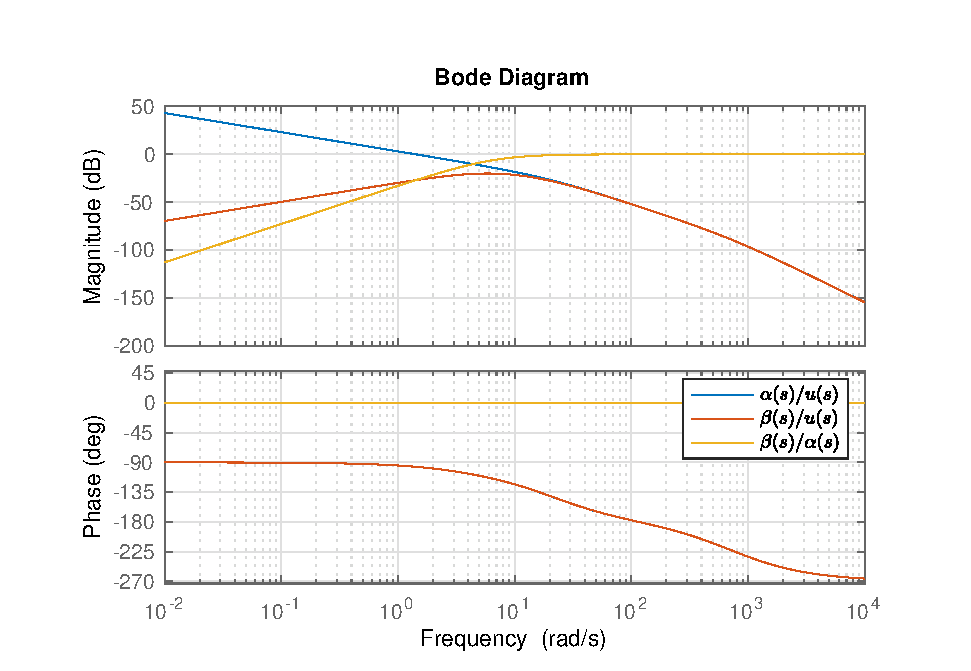
\includegraphics[width = 0.5\textwidth]{figures/bode_all.eps}
    \caption{Bode diagrams of the t.f. \eqref{eq:tf_a_u},\eqref{eq:tf_b_a}, and \eqref{eq:tf_b_u}.}
    \label{fig:bode_all}
\end{figure}
\begin{figure}[h]
\vspace{-0.4cm}
    \centering
    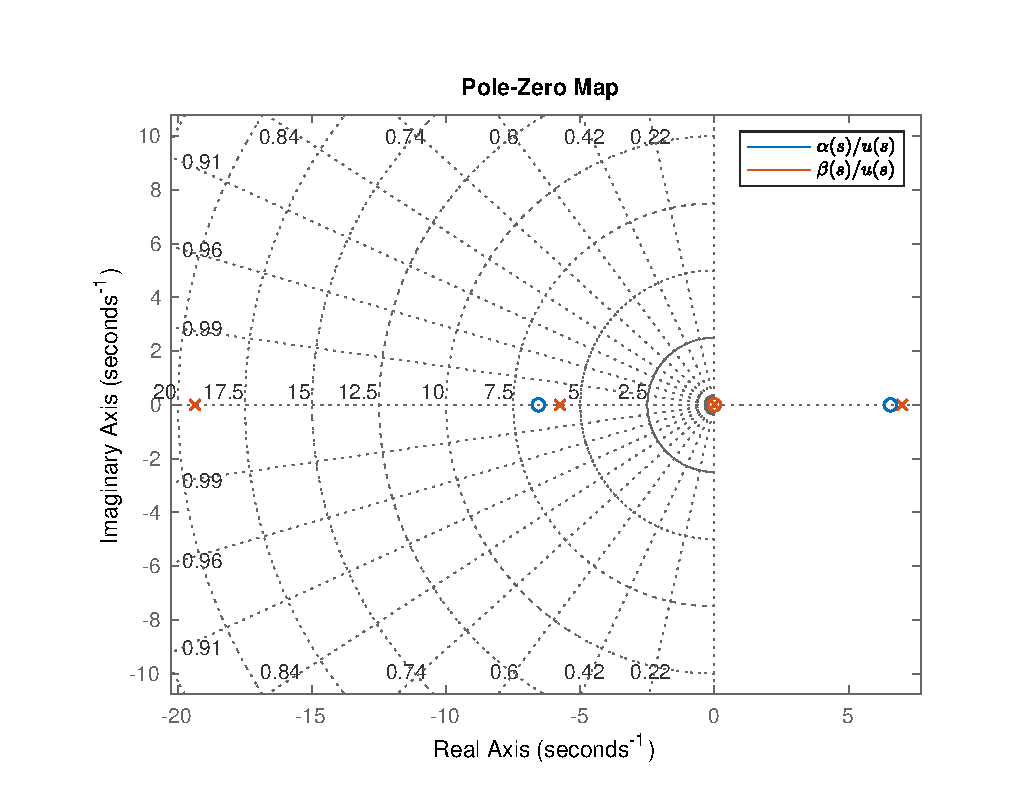
\includegraphics[width = 0.5\textwidth]{figures/pz_all.eps}
    \caption{Pole-zero maps of the t.f. \eqref{eq:tf_a_u} and \eqref{eq:tf_b_u}.}
    \label{fig:pz_all}
\end{figure}

On one hand, consider the t.f. $\alpha(s)/u(s)$. It is noticeable that the gain tends to infinity as $\omega\rightarrow 0$, which is consistent with the presence of an integrator pole on the dynamics of $\alpha$ as put forward in Section \ref{sec:dynModes}. Also, note on Fig. \ref{fig:pz_all} that the two zeros of the t.f. are very close to the pair of real poles associated with the dynamics of the inverted pendulum, given that $\alpha$ is not very affected by the dynamics of the inverted pendulum, but rather on the integrator and pole that models the angular velocity of the DC motor shaft. This analysis is consistent with the claim made on Section \ref{sec:dynModes} about the correspondence between the poles and the dynamics of the physical system. For these reasons, the effect of the inverted pendulum poles is barely visible in the bode plot of the gain. The gain drops asymptotically at $-40$dB/dec after $p = -19.3$ rad/s and at $-60$dB/dec after the pole of the DC motor dynamics, attenuating high input frequencies. Thus, the angle $\alpha$ can only be controlled effectively from the input $u$ on low frequencies limited by the frequency of the pole that models the DC motor shaft angular speed, which makes sense in a physical intuitive perspective. Furthermore, as seen in Section \ref{sec:trck} the existence of a nonminimum phase zero leads to the manifestation of a whiplash effect on the time response of the angle $\alpha$. 

On the other hand, consider the t.f. $\beta(s)/u(s) = (\beta(s)/\alpha(s)) (\alpha(s)/u(s))$. Note that it has two zeros at the origin, one of which cancels with the integrator pole associated with the dynamics of $\alpha$, which is consistent with the asymptotic evolution of $+20$dB/dec at low frequencies. After the frequency of the inverted pendulum poles and the pole that models the DC motor shaft angular speed, the gain drops asymptotically at $-40$dB/dec and at $-60$dB/dec after the pole of the DC motor dynamics, attenuating high input frequencies. It is interesting to point out that, since $\alpha(s)/u(s)$ has low-pass dynamics and $\beta(s)/\alpha(s)$ has high-pass dynamics, the t.f. $\beta(s)/u(s)$ has band-pass dynamics. Thus, the angle $\beta$ can only be controlled effectively from the input $u$ on a limited band of frequencies, centered, approximately, at the characteristic frequency of the inverted pendulum, which makes sense in a physical intuitive perspective.

It is possible to interpret the frequency response of the system to comment on the controllability and observability of the system. First, as it was shown in Section \ref{sec:ctrolbty}, the plant is controllable, despite the fact that the state has five components, two of which are two mechanical degrees of freedom of the physical system. The way the controllability of the system is achieved lies on its frequency response. First, note, for convenience, that for continuous-time systems, controllability is equivalent to the ability to drive the system from any initial position to the origin in finite time \cite[Definition 9.1]{rugh1996linear}. In fact, for the same signal $u$, different frequencies have different effects on $\alpha$ and $\beta$. A component with low frequency only affects $\alpha$ and with a frequency in the aforementioned band affects both $\alpha$ and $\beta$. Thus, it is possible to drive both $\alpha$ and $\beta$, and their derivatives, to zero in finite time. This state can be maintained with $u=0$ and this equilibrium $i$ can, thus, be driven to the origin. 

Second, it is pointed out in Section \ref{sec:obsvlty} that if the output of the system is only the angle $\beta$, then the system is not observable. Analyzing the t.f. \eqref{eq:tf_b_u} there is a pole-zero cancellation at the origin. It is possible to conclude that there is a loss either of controllability, which is already known that it is not the case, or observability. Therefore, in this case, the system is not observable. It is easily seen in this case from $\eqref{eq:tf_b_a}$ that the evolution of $\beta$ does not depend on $\alpha$ or its first derivative, only on the second derivative. It is, thus, evident that there is a loss of information of the evolution of $\alpha$ measuring only $\beta$, which is the reason behind the loss of observability. For instance, the measurement of $\beta$ cannot distinguish if $\alpha$ is stationary or moving with constant velocity, or even if $\alpha$ is constant and equal to $\alpha_0$ or $\alpha$ is constant and equal to $\alpha_1\neq \alpha_0$. 

\begin{comment}
Finally, to check the system's frequency response, transfer functions are necessary. Using the Matlab function \textit{ss2tf}, the state space model can be converted to transfer functions. Because the transfer function maps one input to one output and there are two outputs ($\alpha$ and $\beta$), two transfer functions are obtained. One represents the relationship between the input, $u$, and $\alpha$, while the other represents the relationship between $u$ and $\beta$.
Using the Matlab function \textit{bode}, the frequency response is plotted. Figures show that magnitude and phase of the frequency response of the two obtained transfer functions.
The Bode diagram for $\alpha$ tends to +$\infty$ for a constant input, which is consistent with the motor's angular velocity integrator. The magnitude drops at a rate of -40 dB/dec after the pole at -19.3673, which is related to the torque dynamics in the horizontal bar. Because the poles are very close to the zeros in the transfer function from $u$ to $\alpha$, the change in the phase is negligible.
In the Bode diagram for $\beta$, the zeros in the origin, along with a pole, leads to an increase of 20 dB/dec at low frequencies. This means that the pendulum dynamics are little excited by low frequency inputs in the motor. On the other hand, the dynamics for $\beta$ are excited for high frequencies of $\alpha$ (the dynamics of $\beta$ with an input of $\alpha$ is similar to a high-pass filter) and characterized by two zeros at the origin and the two poles from the pendulum.
It is possible to conclude then that the diagram for $\beta$ is a combination of these two effects: at low frequencies, $u$ excites the horizontal bar, but the horizontal bar does not excite the pendulum; at high frequencies, the horizontal bar's movement excites the pendulum, but the bar itself cannot be excited by the motor. It is concluded that the pendulum can be controlled by an input $u$ with medium frequency.
To conclude this analysis, note that the Bode diagrams confirm the previous analysis of the system's controllability and observability. Earlier, it was shown that the system is controllable. Note that the system has two degrees of freedom that must be controlled: $\alpha$ and $\beta$. The bode diagram for $\alpha$ tends to +$\infty$ because of the integrator. On the other hand, $\beta$ is only sensible to a frequency range around 5 rad/s = 0.8 Hz. So, even if the system has only one input, $\alpha$ and $\beta$ can both be controlled, because, in the frequency domain, each one is controlled differently.
In terms of observability, it is best to look directly at the transfer functions. Previously, it was concluded that measuring only $\beta$ would result in a system that is not observable. Indeed, looking at the transfer function from $u$ to $\beta$
\[\frac{1.915e04 s^2 + 1.981e-13 s + 1.275e-10}{s^5 + 755.4 s^4 + 1.33e04 s^3 - 4.816e04 s^2 - 5.757e05 s}\]
it is possible to verify the occurrence of a pole-zero cancellation at the origin, which leads to a loss of observability. The same does not occur with the transfer function from $u$ to $\alpha$ or with the transfer function from $\beta$ to $\alpha$, which implies that measuring both variables results in an observable system.
Additionally, the pole-zero maps for each transfer function are also plotted and presented below.
\end{comment}

\section{State feedback controller}\label{sec:ctr}
The control strategy synthesis approach followed in this project follows two steps: i) the state feedback controller synthesis; and ii) the state observer synthesis. It is well known that due to the Separation Theorem \cite[Chapter 15]{rugh1996linear}, one can design the state feedback controller assuming that full state feedback is available. In fact, the poles of the closed-loop estimated state feedback system are the reunion of the closed loop poles of the controller and the closed loop poles of the observer. This property is exemplified in Section \ref{sec:obs}.

In Section \ref{sec:ctrolbty}, it was concluded that the LTI system that describes the dynamics of the plant about the upright position is completely controllable. Thus, one can find a gain $\mathbf{K}$ of the state feedback control action
\begin{equation*}
    u = -\mathbf{K x}\:,
\end{equation*}  
such that the closed-loop system poles are wherever one desires. Nevertheless, the approach followed in this project is to select the gain that minimizes the performance index
\begin{equation}\label{eq:idx}
    J := \int_0^\infty (\mathbf{x}^T \mathbf{Q} \mathbf{x} + u^T R u) dt\:,
\end{equation}
where $\mathbf{Q}\succeq \mathbf 0$ and $R \succ 0$ are matrices of appropriate dimensions that weigh, respectively, the state and the input of the system. It is well-known that the computation of the optimal gain is equivalent to solving an Algebraic Ricatti Equation (ARE), which was carried out numerically with appropriate software. This design method is guaranteed to stabilize the closed-loop dynamics \cite[Section 3.2]{anderson2007optimal} of the LTI model for any choice of $\mathbf{Q}\succeq \mathbf 0$ and $R \succ 0$. 

It is necessary to properly select the weighting matrices. First, note that the result of the minimization of the performance index \eqref{eq:idx} remains unchanged if both weighting matrices are multiplied by the same scalar. Thus, without loss of generality, the input weighting matrix is selected to be given by $R = 1$. Second, it was pointed out in Section \ref{sec:dynModes} that the only modes that are not stable are associated with the angle of the horizontal bar, \textit{i.e.}, the dynamics of $\alpha$, and the inverted pendulum dynamics, \textit{i.e.}, the dynamics of $\beta$. Thus, it was decided to weigh only the state variables $\alpha$ and $\beta$. The regulation of $\alpha$ and $\beta$ ensures the regulation of their derivatives, so the states $\dot{\alpha}$ and $\dot{\beta}$ are not weighted. Third, no coupled weights between states were considered, so $\mathbf{Q}$ is diagonal. Also, the diagonal entries were selected such that the performance index $J$ is dimensionless. The matrix $\mathbf{Q}$ is of the form
\begin{equation*}
    \mathbf{Q}\!=\! \gamma\; \mathrm{diag}\!\!\left(1/{\left(k\frac{10\deg}{180 \deg} \pi\right)^2}\!\!,0,{1}/{\left(\frac{10\deg}{180 \deg} \pi\right)^2}\!\!,0,0\!\right),
\end{equation*}
where $\gamma$ is a scaling factor and $k$ is a weighting factor between $\beta$ and $\alpha$.

Before proceeding with the selection of $\gamma$ and $k$, it is important to point out a few characteristics of the approximations and assumptions made up to this point, that have a significant impact on the controller synthesis guidelines. First, it is important to stress that the model used so far for the gain synthesis is only valid for a neighborhood around the upright position of the pendulum. Second, the model parameters are nominal, but there is uncertainty in the identification of the physical and electric parameters of the plant. Third, the LTI model does not take into account the several nonlinear and non-ideal effects that are verified in the physical plant, which are explored extensively in Section \ref{sec:sim}. For these reasons, while it is possible to design, with the LTI model, an infinitely fast controller, which relies excessively on the model dynamics, it will not stabilize the real plant dynamics. It is, thus, of paramount importance to design a robust controller, \textit{i.e}, it is necessary to find a compromise between regulation speed and actuation smoothness, which contributes to the robustness of the controller.

Having these guidelines in mind, the next step is to select $\gamma$ and $k$. For that purpose, a simulation of $T = 10$ s, with $\mathbf{x}_0 = [50\deg\;0 \;10\deg\; 0 \;0]^T$, an impulsive disturbance on the plant input with an amplitude of $A_p = 4$V and duration of $\Delta t_p = 0.2$ s at $t = 5$ s, is considered. The characteristics of the simulations were devised to be representative of the normal operation of the plant. Fig. \ref{fig:LQR_k} depicts the evolution of $\alpha$ and $\beta$ for different values of $k$, with $\gamma = 10$. First, as expected, the greater $k$ is, the lesser the weight given to $\alpha$ and it takes longer for $\alpha$ to converge to zero. Second, while for $k = 0.1$ and $k= 1$, there is significant overshoot of $\beta$, that does not happen for $k = 10$ or $k=100$. For these reasons, the value that leads to the fastest convergence of $\alpha$ and that does not lead to significant overshoot of $\beta$ is selected, \textit{i.e.}, $k = 10$. 
\begin{figure}[h]
    \centering
    \includegraphics[width = 0.5\textwidth]{figures/LQR_k.png}
    \caption{Time response of $\alpha$ and $\beta$ for different values of $k$, with $\gamma = 10$.}
    \label{fig:LQR_k}
\end{figure}
\begin{comment}
\begin{figure}[h]
    \centering
    \includegraphics[width = 0.5\textwidth]{figures/LQR_k_u.png}
    \caption{Plant input for different values of $k$, with $\gamma = 10$.}
    \label{fig:LQR_k_u}
\end{figure}
\end{comment}

Figs. \ref{fig:LQR_gamma} and \ref{fig:LQR_gamma_u} depict the evolution of $\alpha$ and $\beta$ and the plant input, respectively, for different values of $\gamma$, with $k = 10$. First, note that, as expected, the greater $\gamma$ is, the greater weight is given to the state variables in relation to the weight of the input, thus it takes longer to drive the state to zero. Conversely, if $\gamma$ is lowered, the control action becomes more aggressive and the regulation is achieved faster. Second, in this particular simulation, the actuation input is greater, in absolute value, than 5V, which is as put forward in Section \ref{sec:sim} the saturation of the actuation, for $\gamma = 100$ and $\gamma= 1000$. For these reasons, the value that leads to the fastest regulation and that does not lead to actuation input above 5V is selected, \textit{i.e.}, $\gamma = 10$. 
\begin{figure}[h]
    \centering
    \includegraphics[width = 0.5\textwidth]{figures/LQR_gamma.png}
    \caption{Time response of $\alpha$ and $\beta$ for different values of $\gamma$, with $k = 10$.}
    \label{fig:LQR_gamma}
\end{figure}
\begin{figure}[h]
    \centering
    \includegraphics[width = 0.5\textwidth]{figures/LQR_gamma_u.png}
    \caption{Plant input for different values of $\gamma$, with $k = 10$.}
    \label{fig:LQR_gamma_u}
\end{figure}

Table \ref{tb:cl_poles_LQR} depicts the poles of the closed loop system with full state feedback, with the gain synthesized with $k=10$ and $\gamma = 10$. First, as guaranteed by this synthesis technique, the system became stable in closed loop, since all the poles are on the left half complex plane (LHCP). Second, the pole associated with the DC motor dynamics remains almost unchanged. Nevertheless, the remaining four poles were mapped, due to the state feedback, to two pairs of complex conjugate poles, with similar damping coefficients, the slowest of which has a time constant of 0.6s.

\begin{table}[h]
    \centering
    \caption{Poles of closed-loop system with full state feedback.}
    \begin{tabular}{cccc}
         \hline
         Pole & Damping & $\omega$ (rad/s) & Time constant (s) \\\hline
   -7.37e+02  &                1.00e+00  &     7.37e+02   &       1.36e-03    \\
 $-1.89e+01 + 1.15e+01i $    &8.55e-01    &   2.22e+01    &      5.28e-02    \\
 $-1.89e+01 - 1.15e+01i $  &  8.55e-01   &    2.22e+01    &      5.28e-02    \\
 $-1.68e+00 + 1.09e+00i$   &  8.38e-01    &   2.00e+00    &      5.96e-01    \\
 $-1.68e+00 - 1.09e+00i$   &  8.38e-01    &   2.00e+00     &     5.96e-01\\
        \hline
    \end{tabular}
    \label{tb:cl_poles_LQR}
\end{table}



\begin{comment} % Original - fui copiando [Leo]
\hspace{0.5 cm}
The first strategy is a simple state feedback controller, defined by the control law
\begin{equation}
    u(t) = -K x(t)
\end{equation}
where u(t) is the input, x(t) is the state, and K is a vector of gains. When this control law is coupled with the plant model, a new equation for the system's dynamics is obtained
\begin{equation}
    \dot x = (A - BK)x
\end{equation}
In the previous section, it was concluded that the system was controllable. This means it is possible to calculate a vector K such that the eigenvalues of (A - BK) are wherever we desire. In order to calculate K, the Matlab function \textit{lqr} is used. This function minimizes the quadratic cost function
\begin{equation}
    J = \int_0^\infty (x^T Q_r x + R_r u^2) dt
    \label{eqn_3}
\end{equation}
where $R_r$ is a positive scalar and $Q_r$ is a positive semi-definite matrix. Note that it is not necessary to minimize a cost function to obtain K. It is also possible to specify closed-loop eigenvalues and then compute K.
As an example, $R_r$ is set to 5 and $Q_r$ is set to $600*diag([0.1*0.18^2,0,0.18^2,0,0])$. Table \ref{ABK_eig} shows the obtained eigenvalues for the closed loop system.
\begin{table}[h]
    \centering
    \begin{tabular}{|c|c|}
         \hline
        Eigenvalue 1 & -737.3184\\
         \hline 
        Eigenvalue 2 & -19.1116\\ 
         \hline
        Eigenvalue 3 & -8.1361\\
         \hline
        Eigenvalue 4 & -4.9980\\ 
         \hline
        Eigenvalue 5 & -0.8991\\
        \hline
    \end{tabular}
    \caption{Eigenvalues of Matrix (A - BK) for a given example}
    \label{ABK_eig}
\end{table}
Note that the real part of all the obtained eigenvalues is negative, which means that the resulting system is stable. Now that it is verified that the controller works, it is interesting to analyze the impact of the parameters $Q_r$ and $R_r$ on the system's response. For this purpose, two experiments are devised.
First, $Q_r$ is kept constant and $R_r$ is progressively increased. Note, by looking at equation (\ref{eqn_3}), that increasing $R_r$ gives more importance to $u$. However, since the objective is to minimize the cost function, increasing $R_r$ will prioritize smaller values of $u$. What happens in the simulations is that the initial value for $u$ is big (in terms of absolute value), but the transition to smaller values, near zero, is faster as $R_r$ increases.
For the other experiment, $R_r$ is kept constant and $Q_r$ is progressively increased. $Q_r$ is devised as a diagonal, semidefinite matrix, so increasing the matrix means increasing the values of the diagonal. Again, note, by looking at equation (\ref{eqn_3}), that increasing $Q_r$ gives more importance to the state variables, $x$. To minimize the cost function, increasing $Q_r$ will prioritize smaller values of $x$. What happens in the simulations is that, by increasing $Q_r$, the state variables of interest, $\alpha$ and $\beta$, converge to zero more rapidly. As a consequence, $u$ also has more abrupt transitions. 
In theory, it would be possible to make the system infinitely fast. Due to the uncertainties of the system's model, this should not be done. Thus, to get a good controller for the real system, a compromise is needed between fast actuation and fast convergence to the origin.
\end{comment}

\section{State Observer}\label{sec:obs}
In this section, the second and final step of the control strategy synthesis approach followed in this project is addressed, synthesizing an optimal state observer. Such optimal state observer is also known as the Kalman filter. The optimal observer and controller synthesis are dual problems, so, in this project, they are treated in a very similar manner. Consider the LTI model of the plant with zero-mean Gaussian process and sensor noise
\begin{equation*}
\begin{cases}
    \dot{\mathbf{x}} = \mathbf{Ax}+\mathbf{B}u+\mathbf{w}\\
    \mathbf{y} = \mathbf{Cx}+\mathbf{v}
    \end{cases}\:,
\end{equation*}
where $\mathbf{w} \sim \mathcal{N}(\mathbf{0},\mathbf{Q_e})$ is the process noise, and $\mathbf{v} \sim \mathcal{N}(\mathbf{0},\mathbf{R_e})$ is the sensor noise.
Also, consider a continuous-time Luenberger observer 
\begin{equation}\label{eq:luenberguer}
    \dot{\hat{\mathbf{x}}} = \mathbf{A} \hat{\mathbf{x}} + \mathbf{B}u + \mathbf{L}(\mathbf{y} - \mathbf{C}\hat{\mathbf{x}})\:,
\end{equation}
where $\mathbf{L}$ is the observer gain, and $\mathbf{C}$ is given by \eqref{eq:Cused}, such that the system is completely observable. The Kalman gain is computed such that the trace of the covariance of the estimation error is minimum. Analogously to the controller synthesis problem, it is guaranteed that the Kalman gain exists, since the LTI system at hand is observable. 

It is necessary to properly select the covariance matrices to synthesize the observer gain. Even thought the matrices $\mathbf{Q_e}$ and $\mathbf{R_e}$ have a physical meaning, given that it is very difficult to estimate the process covariance in practice, they are often selected empirically, which is the approach followed in this project. First, analogously to the controller synthesis problem, the gain that achieves the minimum trace of the estimation error covariance matrix remains unchanged if both $\mathbf{Q_e}$ and $\mathbf{R_e}$ are multiplied by the same scalar. Thus, without loss of generality, the  $\mathbf{R_e}$ is selected to be
\begin{equation*}
    \mathbf{R_e} = \left(\frac{1\deg}{180\deg}\pi\right)^2\mathbf{I}\:,
\end{equation*}
since it is assumed that both angle sensors have similar additive noise. Second, process noise couplings between state variables is neglected for the observer's synthesis, which, although it is not a good approximation in this case, is a common practice for designing state observers. The process noise covariance matrix is, therefore, chosen to be a diagonal matrix. Third, the entries of matrix $\mathbf{Q_e}$ are selected such that the dimensions and orders of magnitude are consistent. As a result, $\mathbf{Q_e}$ was chosen to be of the form
\begin{equation*}
\begin{split}
    \mathbf{Q_e}\!=\! \phi\; &\mathrm{diag}({\left(\frac{1\deg}{180 \deg} \pi\right)^2}\!\!,{\left(\omega_d^*\frac{1\deg}{180 \deg} \pi\right)^2}\!\!,\\
    &{\left(\frac{1\deg}{180 \deg} \pi\right)^2}\!\!,{\left(\omega_d^*\frac{1\deg}{180 \deg} \pi\right)^2}\!\!,(0.025 \mathrm{A})^2\!),
    \end{split}
\end{equation*}
where $\phi$ is a scaling factor, and $\omega_d^*$ is a characteristic frequency of the time response of $\alpha$ and $\beta$. Fourth, given that the dynamics of both $\alpha$ and $\beta$ are governed by both pairs of complex conjugate closed loop poles presented in Table \ref{tb:cl_poles_LQR}, the characteristic frequency $\omega_d^*$ was chosen to be the damped frequency of the fastest pair of complex conjugate poles. It is, thus, given by $\omega_d^* = \omega_n \sqrt{1-\xi^2} \approx 10$ rad/s, where $\omega_n$ is the natural frequency of the poles and $\xi$ their damping coefficient. Fifth, the larger $\phi$ is, the lower is the reliance on the model, which makes the observer rely more on the measurements taken, which, in turn, leads to faster observer poles. It is also very important to remark that, since the controller and observer are cascaded, the observer should be, at least, four times faster than the controller \cite{J.M.Lemos_1_2019}. Table \ref{tb:speed_r} presents the value of the ratio between the time constants of the slowest poles of the controller and observer. If one selects too high a value for $\phi$, one is relying too much on the sensor's measurements, whose noise leads to a jittery control action. For that reason, one selects the lowest value of $\phi$ in Table \ref{tb:speed_r} that verifies the condition on the speed ratio, \textit{i.e.}, $\phi = 100$.

\begin{table}[h]
    \centering
    \caption{Ratio between the time constants of the slowest poles of the controller and observer, for various values of $\phi$.}
    \begin{tabular}{cccc}
         \hline
         $\phi$ & $T_c/T_o$ \\\hline
            10 & 2.28\\
            100 & 6.05 \\
            1000 & 9.87\\
        \hline
    \end{tabular}
    \label{tb:speed_r}
\end{table}

Fig. \ref{fig:LQG} depicts the evolution of the estimation error, for the designed observer gain and Table \ref{tb:cl_poles_obs} presents the poles of the observer, which, by \eqref{eq:luenberguer}, are given by the eigenvalues of $\mathbf{A}-\mathbf{LC}$. As expected, the estimation error converges to zero and the observer poles are on the LHCP.
\begin{figure}[h]
    \centering
    \includegraphics[width = 0.5\textwidth]{figures/LQG.png}
    \caption{Time response of estimation error of the state variables, with $\phi = 100$.}
    \label{fig:LQG}
\end{figure}
\begin{table}[h]
    \centering
    \caption{Poles of the observer, with $\phi = 100$.}
    \begin{tabular}{cccc}
         \hline
         Pole & Damping & $\omega$ (rad/s) & Time constant (s) \\\hline
-7.37e+02      &           1.00e+00   &    7.37e+02    &      1.36e-03   \\
 -1.06e+01 + 5.76e+00i   &  8.79e-01  &     1.21e+01 &         9.40e-02    \\
 -1.06e+01 - 5.76e+00i  &   8.79e-01     &  1.21e+01   &       9.40e-02   \\ 
 -1.02e+01             &    1.00e+00   &    1.02e+01   &       9.85e-02   \\ 
 -1.99e+01              &   1.00e+00   &    1.99e+01   &       5.04e-02  \\
        \hline
    \end{tabular}
    \label{tb:cl_poles_obs}
\end{table}

Having designed the controller and the observer separately, they can be cascaded together, $i.e.$, using estimated state feedback $u = -\mathbf{K\hat{x}}$. This can be done without loss of stability, for the LTI system, due to the Separation Theorem mentioned beforehand. In fact, writing the estimation error dynamics, one obtains $\dot{\mathbf{e}} = (\mathbf{A}-\mathbf{LC})\mathbf{e}$, from \eqref{eq:luenberguer}, with $\mathbf{e}:=\mathbf{\hat{x}}- \mathbf{x}$. And from the
estimated state feedback control action, $\dot{\mathbf{x}} = (\mathbf{A}-\mathbf{BK})\mathbf{x}-\mathbf{BKe}$. Considering the augmented system of state variables and estimation error, it is easily concluded that the poles of the closed-loop estimated state feedback system are the reunion of the poles of the controller and of the observer. Thus, the stability and modes of the individually synthesized components remain unchanged. Nevertheless, it is important to point out that the transient time responses are inevitably going to change, given that there is no guarantee about the position of the zeros of the closed-loop estimated state feedback system. 

\begin{comment}% o texto do controlador
The control strategy synthesis approach followed in this project follows two steps: i) the state feedback controller synthesis; and ii) the state observer synthesis. It is well known that, due to the Separation Theorem \cite[Chapter 15]{rugh1996linear}, one can design the state feedback controller assuming that full state feedback is available. In fact, the poles of the closed-loop estimated state feedback system are the reunion of the closed loop poles of the controller and the closed loop poles of the observer. This property is exemplified in Section \ref{sec:obs}.
In Section \ref{sec:ctrolbty}, it was concluded that the LTI system that describes the dynamics of the plant about the upright position is completely controllable. Thus, one can find a gain $\mathbf{K}$ of the state feedback control action
\begin{equation*}
    u = -\mathbf{K x}\:,
\end{equation*}  
such that the closed-loop system poles are wherever one desires. Nevertheless, the approach followed in this project is to select the gain that minimizes the performance index
\begin{equation}\label{eq:idx}
    J := \int_0^\infty (\mathbf{x}^T \mathbf{Q} \mathbf{x} + u^T R u) dt\:,
\end{equation}
where $\mathbf{Q}\succeq \mathbf 0$ and $R \succ 0$ are matrices of appropriate dimensions that weigh, respectively, the state and the input of the system. It is well-known that the computation of the optimal gain is equivalent to solving an Algebraic Ricatti Equation (ARE), which was carried out numerically with appropriate software. This design method is guarateed to stabilize the closed-loop dynamics \cite[Section 3.2]{anderson2007optimal} of the LTI model for any choice of $\mathbf{Q}\succeq \mathbf 0$ and $R \succ 0$. 
It is necessary to properly select the weighting matrices. First, note that the result of the minimization of the performance index \eqref{eq:idx} remains unchanged if both weighting matrices are multiplied by the same scalar. Thus, without loss of generality, the input weighting matrix is selected to be given by $R = 1$. Second, it was pointed out in Section \ref{sec:dynModes} that the only modes that are not stable are associated with the angle of the horizontal bar, \textit{i.e.}, the dynamics of $\alpha$, and the inverted pendulum dynamics, \textit{i.e.}, the dynamics of $\beta$. Thus, it was decided to weight only the state variables $\alpha$ and $\beta$. The regulation of $\alpha$ and $\beta$ ensures the regulation of their derivatives, so the states $\dot{\alpha}$ and $\dot{\beta}$ are not weighted. Third, no coupled weights between states were considered, so $\mathbf{Q}$ is diagonal. Also, the diagonal entries were selected such that the performance index $J$ is adimensional. The matrix $\mathbf{Q}$ is of the form
\begin{equation}
    \mathbf{Q}\!=\! \gamma\; \mathrm{diag}\!\!\left(1/{\left(k\frac{10\deg}{180 \deg} \pi\right)^2}\!\!,0,{1}/{\left(\frac{10\deg}{180 \deg} \pi\right)^2}\!\!,0,0\!\right),
\end{equation}
where $\gamma$ is a scaling factor and $k$ is a weighting factor between $\beta$ and $\alpha$.
%% begin original / fui copiando e alterando 
\end{comment}
\begin{comment}
The second strategy is to find the vector of gains of a state observer. The observer's objective is to make an estimation of the state $x$, $\hat{x}$. The observer is defined by the following differential equation

\begin{equation}
    \dot{\hat{x}} = A \hat{x} + B u + L(y - C\hat{x}) 
\end{equation}

Adding the observer to the system's dynamics adds closed-loop poles to the system, which are the eigenvalues of (A - LC).

The vector of gains is designed to achieve zero estimation error. The Kalman filter is used to achieve this goal, using for this the Matlab function \textit{lqe}. Since the observer also uses the gains K of the feedback controller, we decided to use as fixed values the gains obtained in the previous section.
We decided to only consider gains L such that: \\

1) The poles of the observer are at least 4 times faster than those of the controller; \\

2) The absolute value of $u$ must not surpass 5 V; \\

3) The errors of $\alpha$ and $\beta$ should reach a chosen threshold (5\% of their initial values) at a similar time.\\

The initial values for the $Q_e$ and $R_e$ matrix were chosen such that each entry has the same order of magnitude of the corresponding parameter. We then changed one parameter at a time to access its effect on the observer: \\

1) $G$ Matrix: equally increasing the gains of the process noise shifts the slowest pole to the left, leading to a faster observer. However, increasing the gain too much results in the opposite effect, where the slowest pole begins shifting to the right and the observer becomes slower. As the gain increases, there is a faster shift in the motor's actuation, followed by a slower actuation. \textcolor{blue}{Eu não tenho a certeza da segunda frase. Eu multipliquei por 100000 e não fica mais lento. Pelo menos aquela divisão entre os polos mais pequenos continua a aumentar.} \\

2) $Q_e$ Matrix: if all the parameters in the diagonal are raised equally, the same effect of the parameter G occurs; increasing only the parameter in $\beta$ results in a slower observer; increasing only the parameter in $\alpha$ results in a faster observer. \textcolor{blue}{Eu não consigo arranjar uma razão para a última parte. Porque eu pensei que se aumentassemos o fator em alpha ou em beta que ele ia ficar sempre mais lento, visto que estamos a dizer que o modelo não é de confiança.} \\

3) $R_e$ matrix: increasing Re results in a slower observer, as the slowest pole migrates to the right. \textcolor{blue}{Suponho que isto seja porque estamos a dizer que os sensores não são de confiança.}

After these experiments, it was possible to find gain values that satisfy all the required conditions (Table \ref{tab:obs}).

\begin{table}[h]
    \centering
    \begin{tabular}{|c|c|}
    \hline
    Eigenvalue 1 & - 737.32 \\ \hline 
    Eigenvalue 2 & - 7.09 + 2.43 i \\ \hline
    Eigenvalue 3 & - 7.09 - 2.43 i \\ \hline
    Eigenvalue 4 & - 9.26 \\ \hline
    Eigenvalue 5 & - 19.39 \\ \hline
    \end{tabular}
    \caption{Eigenvalues of Matrix (A - LC)}
    \label{tab:obs}
\end{table}

The quotient of the real parts of the slowest pole of the observer and the slowest pole of the estimator is 7.884951, satisfying condition 1).

To observe how the error of $\alpha$ and $\beta$ are evolving over time we developed a Simulink model with a saturation block to guarantee that condition 3) is met. \\

In Fig. \ref{fig:8_hat} we can see that the the error of $\alpha$ decreases exponentially, while the error for $\beta$ has a small oscillatory behavior. This is related to the eigenvalues of the observer: the ones relative to $\alpha$ have a negative real part but the ones relative to $\beta$ are complex conjugate. In this figure we also marked the point where both errors reach the 5\% threshold at the same time.

\textcolor{blue}{Acham que as figuras estão muito pequenas? Na primeira só interessam os primeiros 2 segundos mas não sei se é encortar o range.}

\begin{figure}[h]
    \centering
    \includegraphics[width = 0.5\textwidth]{figures/8_hat.png}
    \caption{Estimation errors of $\alpha$ and $\beta$ for the linear model with a state observer.}
    \label{fig:8_hat}
\end{figure}

In Fig. \ref{fig:8_ui} it's clear that $u$ never reaches the saturation value.

\begin{figure}[h]
    \centering
    \includegraphics[width = 0.5\textwidth]{figures/8_u_i.png}
    \caption{$u$ and $i$ inputs using the state observer.}
    \label{fig:8_ui}
\end{figure}

To confirm the separation theorem we calculated the eigenvalues of the dynamics matrix of the global system (controller + observer):

\begin{equation*}
\begin{bmatrix}
A & -bK \\
LC & A-LC-bK
\end{bmatrix}
\end{equation*}

As expected, these are the made up by the values in tables \ref{ABK_eig} and \ref{tab:obs}.

\textcolor{blue}{Leo querias também um conjunto de valores que desse anseira. Temos três possibilidades: ou tiramos o bloco de saturação e arranjamos um valor q dê para explodir com aquilo, ou escolhemos valores para os quais o observador é menos de 4 vezes mais rápido do q o controlador, ou escolhemos valores para os quais os thresholds são atingidos em alturas muitos distintas. Qual preferes? Os três é um bocado puxado. Eu vou arranjar valores para cada um deles individualmente.}
\end{comment}
\begin{comment}
\textcolor{red}{SHOW THE EIGENVALUES OF (A - LC) AND (A - BK) FOR A GIVEN DESIGN TO SHOW THAT THE SEPARATION THEOREM IS VERIFIED}
\textcolor{red}{MENTION THE OBSERVER POLES ARE AT LEAST 4 TIMES FASTER THAN THE SYSTEM'S POLES}
For both strategies, Simulink models are developed to observe what happens to the controlled system in both cases.
\end{comment}


% Nova pagina só para ajudar a escrever (depois tira se)

\section{Simulation Results}\label{sec:sim}
Given the impossibility to simulate the controller and observers synthesized in the previous sections on the real system, the plant simulation has to be complemented to include non-ideal effects to allow for a realistic simulation. 

\subsection{Nonlinear simulation model} \label{sec:nonlin}
In Sections \ref{sec:ctr} and \ref{sec:obs}, for the LTI model of the plant, it appears there is no limit on the performance of the controller and observer, which does not portray accurately the dynamics of the plant. The inclusion of nonlinear effects in the plant simulation allows to understand the physical limitations of the plant and to guide the synthesis of a control solution that is robust to such effects. The nonlinear effects considered are: i) nonlinear kinematics; ii) actuator saturation; iii) actuator dead zone; and iv) process and sensor noise. These are presented sequentially, as a means of understanding their impact on the plant response and on the gain synthesis. For that purpose, a simulation of $T = 10$ s, with $\mathbf{x}_0 = [50\deg\;0 \;10\deg\; 0 \;0]^T$, an impulsive disturbance on the plant input with an amplitude of $A_p = 4$V and duration of $\Delta t_p = 0.2$ s at $t = 5$ s,  $\gamma = 10$, $k =10$ and $\phi = 10^2$, is considered, which corresponds to the same simulation and control solution synthesis put forward in Sections \ref{sec:ctr} and \ref{sec:obs}.

\subsubsection{Nonlinear kinematics} First, instead of the LTI system, the simulation was performed with the nonlinear kinematics of the plant, modeled by equation (2.19) in \cite{balula2016nonlinear}, which is shown and compared with the LTI simulation in Fig. \ref{fig:9_1_angles}. It is visible that, for small angles of $\beta$ the linear model is quite accurate, which was expected since the LTI model was obtained from a linearization around $\beta = 0 \deg$. However, as $\beta$ reaches higher values, the time responses begin to differ. In fact, while for the LTI system, one had guarantees about the stability of the controller and observer, that is no longer the case for the nonlinear system. In fact, although the closed-loop system dynamics linearized around $\beta = 0$ are stable, which means that it is an asymptotically stable equilibrium of the nonlinear system, a high enough disturbance or tracking reference on $\alpha$ can easily destabilize the plant. 
\begin{figure}[h]
    \centering
    \includegraphics[width = 0.5\textwidth]{figures/9_1_angles.png}
    \caption{Time response of $\alpha$ and $\beta$ for the nonlinear kinematics.}
    \label{fig:9_1_angles}
\end{figure}

\subsubsection{Actuator saturation} Second, a saturation of $u_{sat} = 5$V, which corresponds to the actual saturation of the physical plant, was included. Figs. \ref{fig:9_2_angles} and \ref{fig:9_2_u} show the evolution of $\alpha$ and $\beta$ and the actuator input, respectively, and their comparison with the evolution that would be obtained without saturation. It is concluded that, although the actuator is saturated for a very short duration, the effect on the time response is quite significant, leading to a significant increase of the settling time. This effect penalizes aggressive controllers and imposes a limitation on the regulation performance.

\begin{figure}[h]
    \centering
    \includegraphics[width = 0.5\textwidth]{figures/9_2_angles.png}
    \caption{Time response of $\alpha$ and $\beta$ with input saturation.}
    \label{fig:9_2_angles}
\end{figure}
\begin{figure}[h]
    \centering
    \includegraphics[width = 0.5\textwidth]{figures/9_2_u.png}
    \caption{Plant input with input saturation.}
    \label{fig:9_2_u}
\end{figure}

\subsubsection{Dead zone} Third, a very common and important non-linearity of DC motors is their dead-zone. If the interval of the dead-zone is known accurately, it can be easily inverted, which attenuates its effect. However, since it is not easy to estimate it accurately, and given that it varies with time, it was assumed that the dead-zone interval is unknown and equal to $u_{dz} = 0.2[-1;1]$V. Figs. \ref{fig:9_3_angles} and \ref{fig:9_3_u} show the evolution of $\alpha$ and $\beta$ and the actuator input, respectively, and their comparison with the evolution that would be obtained without actuator dead-zone. The introduction of the dead-zone inhibits the effect of small input voltages to the DC motor. Thus, at the equilibrium point $\beta = 0$, the controller has no authority, and the linearized dynamics correspond to the dynamics of the open loop plant, which are known to be unstable. Thus, with the inclusion of the actuator dead-zone the equilibrium point $\beta = 0$ of the nonlinear system is no longer stable, even with a state feedback controller. Nevertheless, once the actuator gets out of the dead-zone, it acts to return the plant to $\beta = 0$. For this reason, either the dead-zone is too large and the controller is unable to return the pendulum to the upright position with a given saturation, or it is able to do so resulting in an oscillatory time response, which can be seen in Fig. \ref{fig:9_3_angles}. Therefore, more aggressive controllers allow to exit the dead-band for a smaller perturbation on $\beta$, and thus achieve better regulation.

\begin{figure}[h]
    \centering
    \includegraphics[width = 0.5\textwidth]{figures/9_3_angles.png}
    \caption{Time response of $\alpha$ and $\beta$ with actuator dead-zone.}
    \label{fig:9_3_angles}
\end{figure}
\begin{figure}[h]
    \centering
    \includegraphics[width = 0.5\textwidth]{figures/9_3_u.png}
    \caption{Plant input with with actuator dead-zone.}
    \label{fig:9_3_u}
\end{figure}

\subsubsection{Process and sensor noise} Lastly, process and sensor noise were modeled as zero-mean Gaussian distributions with covariance matrices \phantom{mmmmmmmmmmmmmmmmmmmmm} $\mathbf{Q_p}\!\!=\!\!10^2\mathrm{diag}(0.018^2,(0.18)^2,(0.018)^2,(0.18)^2,0.025^2)$ and $\mathbf{Q_s} = 0.036^2\mathbf{I}$, respectively. Note that this corresponds to a standard deviation of $\sigma_s \approx 1 \deg$ on the sensors that measure the angle of the bars. Figs. \ref{fig:9_4_angles} and \ref{fig:9_4_u} show the evolution of $\alpha$ and $\beta$ and the actuator input, respectively, and their comparison with the evolution that would be obtained without noise. It is visible that there was a loss of regulation performance as well as an increase on jitteriness of the actuator input.

\begin{figure}[h]
    \centering
    \includegraphics[width = 0.5\textwidth]{figures/9_4_angles.png}
    \caption{Time response of $\alpha$ and $\beta$ with process and sensor noise.}
    \label{fig:9_4_angles}
\end{figure}
\begin{figure}[h]
    \centering
    \includegraphics[width = 0.5\textwidth]{figures/9_4_u.png}
    \caption{Plant input with process and sensor noise.}
    \label{fig:9_4_u}
\end{figure}

\subsection{Performance evaluation}\label{sec:optPer}
To objectively evaluate the regulation performance of the controller on the plant with nonlinear effects, a cost function of the sum of the squared error on the angles $\alpha$ and $\beta$, i.e.,
\begin{equation*}
    \bar{J} = \int_0^T \alpha(t)^2+\beta(t)^2\:,
\end{equation*}
is considered. From the analysis conducted in the previous subsection it was possible to conclude that the nonlinear effects introduce performance limitations. In fact, on one hand, the saturation on the plant input imposes the use of a not too aggressive controller to keep the desired inputs outside the saturation region. On the other hand, the more aggressive the controller is, the less effect the dead-zone has and the quicker the state variables are regulated. In this sense, one has to find a compromise between these two different effects. For that reason, $\bar{J}$ was computed for various combinations of controller and observer gains and it is shown in Fig. \ref{fig:9_5_mesh}. 

\begin{figure}[h]
    \centering
    \includegraphics[width = 0.5\textwidth]{figures/9_5_mesh.png}
    \caption{Regulation cost function for various controllers and observers.}
    \label{fig:9_5_mesh}
\end{figure}

First, it is visible that there are combinations of controller and observer gains that destabilize the closed loop system, which correspond to the green and yellow \textit{plateaus} in Fig. \ref{fig:9_5_mesh}. As discussed in the previous subsection, the nonlinear effects can easily destabilize the closed loop dynamics if the gains are not synthesized robustly and with awareness of the effects. Second, as put forward in Section \ref{sec:obs}, it is necessary that the observer is at least four times faster than the controller. The combinations of controller and observer gains which do not follow this constraint are represented in the orange region of the surface of Fig. \ref{fig:9_5_mesh}. It is visible that, in this region, the system does not become, generally, unstable, but the regulation performance degrades significantly. Third, one can easily find the couple of controller and observer gains that minimizes the cost function, which is represented by the red star in Fig. \ref{fig:9_5_mesh}. The minimum corresponds to $\gamma = 316.2$ and $\phi = 100.0$. Figs. \ref{fig:9_4_angles} and \ref{fig:9_4_u} show the evolution of $\alpha$ and $\beta$ and the actuator input for the optimal solution, respectively, and their comparison with the evolution that was obtained in the previous section. It is visible that there was a clear improvement on the perturbation disturbance properties of the control solution. It is also noticeable that the optimal solution is quite aggressive, which allows to attenuate the effect of the dead zone. Table \ref{tb:cl_poles} shows the poles of the optimal closed loop solution. It is possible to conclude that there are two complex conjugate pairs of poles and the real pole of the DC motor dynamics, which is very fast, remains close to its open loop position.

\begin{figure}[h]
    \centering
    \includegraphics[width = 0.5\textwidth]{figures/9_5_angles.png}
    \caption{Time response of $\alpha$ and $\beta$ of the optimal solution.}
    \label{fig:9_6_angles}
\end{figure}
\begin{figure}[h]
    \centering
    \includegraphics[width = 0.5\textwidth]{figures/9_5_u.png}
    \caption{Plant input with of the optimal solution.}
    \label{fig:9_6_u}
\end{figure}

\begin{table}[h]
    \centering
    \caption{Eigenvalues of the optimal closed loop system.}
    \begin{tabular}{cccc}
         \hline
         Pole & Damping & $\omega$ (rad/s) & Time constant \\\hline
 $-7.37e+02$            &   1.00e+00      & 7.37e+02       &   1.36e-03    \\
 $-3.75e+01 + 3.44e+01i $    &7.37e-01   &    5.08e+01     &     2.67e-02    \\
 $-3.75e+01 - 3.44e+01i  $ &  7.37e-01    &   5.08e+01     &     2.67e-02    \\
 $-1.54e+00 + 1.38e+00i $  &  7.45e-01    &   2.07e+00  &        6.49e-01    \\
 $-1.54e+00 - 1.38e+00i$  &   7.45e-01    &   2.07e+00     &     6.49e-01 \\
        \hline
    \end{tabular}
    
    \label{tb:cl_poles}
\end{table}



\subsection{Disturbances and integral action}\label{sec:dis}
Apart from the nonideal effects considered in Section \ref{sec:nonlin}, it also important to consider an additional two nonideal effects: i) the model identification uncertainty; and ii) constant disturbances.

\subsubsection{Model uncertainty} The model that describes the physical plant depends on a set of physical and electrical parameters that are identified performing a set of experiments on the plant. Although this project does not cover such procedure, it is still important to take into account the uncertainty of the parameters. The uncertainty of the parameters of the plant under study is presented in \cite{balula2016nonlinear}. To study the effects of this uncertainty the optimal solution obtained in Section \ref{sec:optPer} is simulated with uncertainty in the physical and electrical parameters of the network. Each parameter was obtained from a Gaussian distribution with mean of the nominal value of the parameter and standard deviation presented in \cite{balula2016nonlinear}. The evolution of the angles for this simulation is shown is Fig. \ref{fig:10_0_angles}. It is visible that the identified parameters are very accurate, because there is no visible impact on the time evolution of $\alpha$ or $\beta$. Nevertheless, as aforementioned, the plant dynamics have an integrator, which guarantees that even in the presence of substantial model uncertainty, as long as the system remains stable, $\alpha$ is regulated to zero, or, considering the tracking problem, there is no steady-state error because of this effect. All the simulations presented from this point include parameter uncertainty.

\begin{figure}[h]
    \centering
    \includegraphics[width = 0.5\textwidth]{figures/10_0_angles.png}
    \caption{Time response of $\alpha$ and $\beta$ with identification uncertainty.}
    \label{fig:10_0_angles}
\end{figure}

\subsubsection{Disturbances} Another important aspect to take into account are disturbances. Impulsive disturbances were studied in Section \ref{sec:nonlin}, and the controller successfully attenuates such perturbations. Furthermore, there can also be constant (or slowly time-varying) disturbances either i) at the output of the plant, or ii) at the input. For this plant in particular, a constant disturbance on $\alpha$ at the output of the plant is successfully rejected because of the presence of the integrator in the plant dynamics. Nevertheless, there can also be a constant disturbance at the input of the plant, caused, for instance, by a bias on the DC motor amplifier. Consider that the motor amplifier has a bias of $u_{bias} = 0.2$V. Fig. \ref{fig:10_1_angles} shows the evolution of $\alpha$ and $\beta$ in these conditions and it is compared with the evolution without DC motor amplifier bias. It is evident that the controller is unable to reject this constant disturbance and the angle $\alpha$ is not regulated to close to zero.

\begin{figure}[h]
    \centering
    \includegraphics[width = 0.5\textwidth]{figures/10_1_angles.png}
    \caption{Time response of $\alpha$ and $\beta$ with a bias on the DC motor amplifier.}
    \label{fig:10_1_angles}
\end{figure}

The poor performance in the presence of such disturbance suggests the need to include integral action. Consider a new state variable $x_I$ defined by the differential equation $\dot{x_I} = \mathbf{C}_{\alpha}\mathbf{x}-0$, with $\mathbf{C}_{\alpha} = [1\;0\;0\;0\;0]$, \textit{i.e.}, an integrator of the regulation error, and a new control action $u = -\mathbf{Kx}-K_Ix_I$. The augmented dynamics are, thus, given by 
\begin{equation}\label{eq:intSys}
    \dot{\begin{bmatrix}x \\x_I \end{bmatrix}} = \mathcal{A}\begin{bmatrix}x \\x_I\end{bmatrix}+\mathcal{B}u\:,
\end{equation}
where 
\begin{equation*}
    \mathcal{A}:= \begin{bmatrix}\mathbf{A} & 0 \\ \mathbf{C}_{\alpha} & 0 \end{bmatrix} \quad \text{and} \quad \mathcal{B}:= \begin{bmatrix}\mathbf{B} \\ 0 \end{bmatrix}\:.
\end{equation*}
The same controller synthesis procedure may be used to synthesize a gain for the augmented system \eqref{eq:intSys} including the integral action. For this purpose, an augmented matrix $\mathcal{Q}$ is chosen 
\begin{equation*}
    \mathcal{Q} = \mathrm{diag}(\mathbf{Q}^{opt},\mathbf{Q}^{opt}_{11}/100)\:,
\end{equation*}
where $\mathbf{Q}^{opt}$ is the state weighting matrix found to be optimal in Section \ref{sec:optPer}.   
Note that the weight of the integral state was chosen to be two orders of magnitude below the weight of $\alpha$, such that the previously designed poles are not very affected, but rejection of constant (or slowly time-varying) disturbances is achieved. The poles of the closed-loop system obtained with this this design approach are shown in Table \ref{tb:cl_poles_int}. Comparing Tables \ref{tb:cl_poles} and \ref{tb:cl_poles_int}, it is possible to conclude that, as desired, the closed loop poles remain very close to those obtained before the addiction of integral action. Fig. \ref{fig:10_2_angles} shows the evolution of $\alpha$ and $\beta$ with integral action and amplifier bias and it is compared with the evolution without DC motor amplifier bias. The controller is now able to regulate the angle $\alpha$, and a performance similar to the optimal synthesis is achieved. 

\begin{table}[h]
    \centering
    \caption{Eigenvalues of the closed loop system with integral action.}
    \begin{tabular}{cccc}
         \hline
         Pole & Damping & $\omega$ (rad/s) & Time constant (s) \\\hline
 $-7.37e+02   $             & 1.00e+00    &   7.37e+02   &       1.36e-03   \\ 
 $-3.75e+01 + 3.44e+01i $ &   7.37e-01    &   5.08e+01    &      2.67e-02   \\ 
 $-3.75e+01 - 3.44e+01i  $ &  7.37e-01    &   5.08e+01     &     2.67e-02   \\ 
 $-1.53e+00 + 1.39e+00i  $  & 7.41e-01    &   2.07e+00   &       6.52e-01   \\ 
 $-1.53e+00 - 1.39e+00i $  &  7.41e-01    &   2.07e+00    &      6.52e-01  \\  
 $-3.16e-01      $        &   1.00e+00     &  3.16e-01    &      3.16e+00\\
        \hline
    \end{tabular}
    
    \label{tb:cl_poles_int}
\end{table}

It is important to note that the transient response after the pulse became significantly worse with the addition of integral action. Although in this case, for a relatively small disturbance, the system remains stable, for more significant disturbance pulses, or significant changes in the tracking angle of the tracking problem, that is not true. A well-known solution to this problem is the use of an integrator anti-windup technique, described, for instance, in \cite{frazzoli}. The block diagram of the proposed solution is presented in Fig. \ref{fig:blk_diag}, in which the integral state variable is limited to $\pm 0.3$ rad s.

\begin{figure}[h]
    \centering
    \includegraphics[width = 0.5\textwidth]{figures/10_2_angles.png}
    \caption{Time response of $\alpha$ and $\beta$ with a bias on the DC motor amplifier and integral action.}
    \label{fig:10_2_angles}
\end{figure}

\begin{figure}[h]
    \centering
    \includegraphics[width = 0.5\textwidth]{figures/block_diag.png}
    \caption{Block diagram of the controller with integral action.}
    \label{fig:blk_diag}
\end{figure}

\section{Reference Tracking}\label{sec:trck}

The tracking problem is now considered, in which the goal is to follow piece-wise constant reference signals with $\alpha$. To extend the results and synthesis procedure of Section \ref{sec:dis}, a suitable feedforward control action is devised to achieve null steady state error without the presence of the bias on the DC motor amplifier, and the integral state is redefined. 

Consider a control action of the form  $u = -\mathbf{Kx}-K_Ix_I+N\alpha_{ref}$, where $N$ is the feedforward gain and $\alpha_{ref}$ is the piece-wise constant reference signal. The state and integral action feedback gains are those synthesized in Section \ref{sec:dis}, achieving the closed-loop poles in Table \ref{tb:cl_poles_int}. First, neglect the presence of the integral action feedback term. Following the usual procedure, put forward in the course lectures, the transfer function is given by
\begin{equation*}
    \frac{\alpha(s)}{\alpha_{ref}(s)} = \mathbf{C}_{\alpha}(s\mathbf{I}-(\mathbf{A}-\mathbf{BK})^{-1})\mathbf{B}N\:.
\end{equation*}
Given that the closed-loop system is stable (assuming that the non-ideal effects do not destabilize the system), then one can make use of the Finite-Value Theorem, to find the static gain $G_0 =- \mathbf{C}_{\alpha}(\mathbf{A}-\mathbf{BK})^{-1}\mathbf{B}N$. To achieve unitary static gain in these conditions, then, one ought to select 
\begin{equation}\label{eq:N}
    N = -1/(\mathbf{C}_{\alpha}(\mathbf{A}-\mathbf{BK})^{-1}\mathbf{B})\:.
\end{equation}
Before continuing, it is important to remark that although it may seem from \eqref{eq:N} that the value of $N$ is not robust as far as uncertainty in the model is concerned, that is not actually the case. It is easy to verify that due to the presence of an integrator pole in the plant dynamics, the structure of matrix $\mathbf{A}$ is such that, for variations of physical and electrical parameters in relation to the nominal values, unitary $G_0$ is achieved. Finally, to reject the bias on the DC motor amplifier, the integral state is redefined, using the differential equation $\dot{x_I} = \mathbf{C}_{\alpha}\mathbf{x}-\alpha_{ref}$. 

Before proceeding it is important to point out that the use of a feedforward term in the control action is not necessary as far as ensuring an unitary static gain is concerned. In fact, the presence of the integral term achieves unitary static gain, if the system remains stable. Nevertheless, abrupt changes in the reference signal, which are very common in piece-wise constant signals, require significant changes in the steady-state value of the integral state $x_I$. This consequence is very undesirable, not only because it leads to significant overshoot, but can also destabilize the system. For that reason, with the addition of the feedforward control action, the integral state is only such that constant (or slowly time-varying perturbations) are rejected. The integral state anti-windup technique can, then, be used, as in the previous section, to limit integral control action. Fig. \ref{fig:blk_track} depicts the block diagram of the proposed tracking solution. 

\begin{figure}[h]
    \centering
    \includegraphics[width = 0.5\textwidth]{figures/block_trck.png}
    \caption{Block diagram of the controller with integral action for the tracking problem.}
    \label{fig:blk_track}
\end{figure}

Figs. \ref{fig:11_1_angles} and \ref{fig:11_1_u} show the evolution of the angles $\alpha$, $\beta$, and the reference $\alpha_{ref}$, and the control action, respectively. First, it is possible to confirm that the proposed control solution successfully tracks the piece-wise constant reference signal. Second, it is also worth pointing out that the transient response has no noticeable overshoot, because of the anti-windup scheme that was implemented. Third, the presence of a nonminimum phase zero, as pointed out in Section \ref{sec:dynModes}, is very evident in this time response. In fact, every time there is an abrupt change in the reference signal, there is a whiplash effect on the evolution of angle $\alpha$. Fourth, it is possible to conclude that the input is such that it does not reach saturation, but is aggressive enough to achieve good performance in the presence of a dead zone. This is only possible due to the thorough control solution synthesis performed in Sections \ref{sec:ctr} and \ref{sec:obs}, which was adjusted afterwards taking into account the non-ideal effects of the real plant, in Section \ref{sec:sim}.  

\begin{figure}[h]
    \centering
    \includegraphics[width = 0.5\textwidth]{figures/11_1_angles.png}
    \caption{Time response of $\alpha$ and $\beta$ with process and sensor noise.}
    \label{fig:11_1_angles}
\end{figure}
\begin{figure}[h]
    \centering
    \includegraphics[width = 0.5\textwidth]{figures/11_1_u.png}
    \caption{Plant input with process and sensor noise.}
    \label{fig:11_1_u}
\end{figure}

\section{Conclusion}\label{sec:concl}
In this project, a control solution for an inverted pendulum is proposed. Although its dynamics are nonlinear, the control solution synthesis procedure followed makes use of the LTI model of the linearized pendulum about the upright position. A regulation strategy is proposed, which is then extended to the tracking problem, both yielding good performance. First, the plant was characterized in terms of its dynamic modes, where a correspondence was established between the poles of the LTI model and the physical interactions of the real plant. Second, the system was analyzed in terms of controllability and observability, having concluded that it is controllable about the upright position, and, if the angles of both bars are measured, it is observable. Third, the frequency response of the LTI model was analyzed as well. It gave insights into the reason why the system can be controlled with a single input, and why it is necessary to measure the angle of the horizontal bar for the system to be observable. Fourth, the control solution was divided into two design problems: i) the controller with full state feedback; and ii) the state observer. The Separation Theorem guarantees that, when cascaded, the estimated state feedback system remains stable. Although it is possible to design an infinitely fast controller for the LTI model, it is not realist for the application in the real plant. Thus, a compromise between a fast and robust controller is made. Fifth, the state observer is designed to regulate the state estimation error dynamics as fast as possible. Given that the sensor measurements are contaminated with noise, the observer is designed to achieve a compromise between speed and robustness to sensor noise. Sixth, several non-ideal dynamics were taken into account, and their effects were analyzed individually to assess their impact on the control solution design. Seventh, considering a cost index, the previously designed gains were recomputed to mitigate the non-ideal effects, yielding a significant improvement in regulation performance. Eighth, it was shown that the control solution is insensitive to model identification uncertainty, impulsive perturbations, and slowly time-varying disturbances on the output. Integral action was added to the control solution as a means of rejecting a constant bias on the DC motor amplifier that could not be rejected otherwise. Finally, the regulation problem was extended to track piece-wise constant signals with the angle of the horizontal bar. A control solution based on both feedback and feedforward components is proposed, yielding good tracking performance.

\printbibliography

\end{document}

